% LaTeX style file for Ph.D. thesis document
% Institution: Kyungpook National University (KNU)
% 
% (c) Gwenaelle Cunha Sergio (gwena.cs@gmail.com)
% and
% (c) Dennis Singh Moirangthem (mdennissingh@gmail.com)
%
% Please note:
%    1. Compile with XeLatex
%    2. This was not made for monetary purposes and it is free for anyone to use. However, if you do use it or modify it, please acknowledge this work by mentioning this original source code.
%

% !TeX program = lualatex

\documentclass[12pt]{report}

\usepackage{thesis}
%%%%%%%%%%%%%%%%%%%%%
% Required packages %
%%%%%%%%%%%%%%%%%%%%%

% Document formatting
\usepackage{adjustbox}
\usepackage{ragged2e}
\usepackage{setspace}
\usepackage{times}
\usepackage{latexsym}
\usepackage{url}
\usepackage{etoolbox}
\usepackage{graphicx}
\usepackage{url}
\usepackage{amsmath}
\numberwithin{equation}{chapter}
\usepackage{amssymb}
%\usepackage{subfigure}
\usepackage{color}
\usepackage{multirow}
\usepackage{comment}
\usepackage{pdflscape}
\usepackage{bibentry}
\usepackage{caption}
\usepackage{booktabs}
\usepackage[noadjust]{cite}
\usepackage{fancyhdr}


% Needed for \phantomsection definition
\usepackage{hyperref}

% Images
\usepackage{graphicx}
\usepackage{subfig}

% Indents first paragraph
\usepackage{indentfirst}

\usepackage{titlesec}

\usepackage[]{algorithm2e}

\titleformat{\chapter}[display]
{\normalfont\bfseries}{}{0pt}{\Huge}
\setlength\parindent{0pt}

\newtheorem{defn}{Definition}

% Suppress badness warnings
\hbadness=99999

\DeclareMathOperator*{\argmax}{arg\,max}
\DeclareMathOperator*{\argmin}{arg\,min}
\DeclareMathOperator*{\softmax}{softmax}
\DeclareMathOperator*{\aggr}{\boxplus}
\newcommand{\norm}[1]{\left\lVert#1\right\rVert}


%%%%%%%%%%%%%%%%%%%%%%%%
% Document starts here %
%%%%%%%%%%%%%%%%%%%%%%%%
\begin{document}
	
	
\onehalfspacing
\makecover
\makeinnercover\newpage
\pagenumbering{arabic}
%\thispagestyle{empty}
\addtocounter{page}{1}
\tableofcontents \newpage
\listoffigures \newpage

\setstretch{1.0}
\phantomsection~\label{sec:ref}
\addcontentsline{toc}{section}{Summary of Notation} \pagebreak

%%%%%%%%%%%%%%%%%%%%
% Rest of document %
%%%%%%%%%%%%%%%%%%%%
\setcounter{figure}{0}
\setcounter{table}{0}
\setcounter{equation}{0}
\section{Introduction}~\label{sec:introduction}
This is the template
 \pagebreak
\setcounter{figure}{0}
\setcounter{table}{0}
\setcounter{equation}{0}
\chapter{Motivation}~\label{chap:rl_for_seg} \pagebreak

\setcounter{figure}{0}
\setcounter{table}{0}
\setcounter{equation}{0}
\chapter{Preliminaries}~\label{sec:preliminaries}

\section{Image segmentation}~\label{sec:prel_imagesegmentation}

Image segmentation or image partitioning is defined as the process of dividing a digital image into sets of pixels known as the objects in the image.\\
There are many variations concerning the segmentation method itself as well as the goal that is to be achieved. With the rise of CNNs, nowadays these methods are usually fully or by parts learning based. That means, that some parameterized function is optimized in order to approximate some target which can only be described by prior knowledge and/or by drawing samples from a target distribution. For the task of image segmentation these samples are of the form $(x, y)$ which is a realization of a random variable $(X, Y)$ with probability distribution $P_{X, Y}(x, y)$. Samples represent the raw input image $x$ that is to be segmented and the desired segmentation $y$ also referred to as label or label image. The goal is to learn a function $f(x)$ such that it approximates $\mathbb{E}[Y|X=x]$ at best. Since $P_{X, Y}$ is initially not known and only few samples and/or some prior knowledge on its properties are available, the approximation can only be achieved by the Monte Carlo estimate of the expectation obtained from those samples and by dexterous use of the prior knowledge. \\
Some of the variations of learning based methods for image segmentation are distinguished by their level of supervision during the optimization. This is mainly defined by the amount of data samples and prior knowledge on the distribution $P_{X, Y}$ that is available and used by the method.

\begin{itemize}
	\item \textbf{supervised segmentation} is the highest level of supervision. Here only samples from $P_{X, Y}$ are available to the method. If enough samples are available such that all regions in the domain of the distribution are covered sufficiently, this is usually all one needs to arrive at a satisfactory result. However for most applications the set of available samples is very limited.
	\item \textbf{unsupervised segmentation} is the lowest level of supervision. Here no samples from $P_{X, Y}$ are available to the method. The optimization method has to completely rely on prior knowledge on the underlying distribution. Realizations of $X$ are usually still available and can be used for the learning process.
	\item \textbf{semi-supervised segmentation} is the transition between the previous two. Similar to supervised learning, semi-supervised learning uses samples from $P_{X, Y}$, but not only. There are also realizations of $X$ available as well as some prior knowledge on $P_{X, Y}$ which is used for the learning process.
	\item \textbf{self-supervised learning} is usually referred to when the method generates some kind of supervisory signal for itself. E.g. an automated labeling procedure to generate sample approximations $(x, \bar{y})$. Self-supervised learning is a special case of unsupervised learning.
\end{itemize}

Other variations that focus more on the goal that should be achieved are

\begin{itemize}
	\item \textbf{semantic segmentation} is the process of assigning class labels to each pixel in the image. Different objects instances of the same class are labeled equally. Usually only some object classes of interest get a unique class label assigned to. All other object classes receive the label background.
	\item \textbf{instance segmentation} is similar to semantic segmentation in the sense that each pixel in the image is assigned a label to. This label attributes a pixel either to background or to an instance of an object class. Therefore different objects of the same class are labeled differently. Here the label of an instance is also referred to as object id.
	\item \textbf{panoptic segmentation} is a fusion of the previous two. For all pixels belonging to instances of some defined set of classes, instance segmentation is performed. For the remaining pixels, semantic segmentation without a background label is performed. The object instances for which instance segmentation is performed are referred to as "things" (objects with a well defined shape like cars, buildings ...) and the object instances for which semantic segmentation is performed are referred to as "stuff" (background regions like grass, sky ...).
\end{itemize}
\section{Reinforcement Learning (RL)}~\label{ssec:rl}
Please note that this is an aggressively shortened summary. For a deeper introduction please refer to \cite{SB_all}.
The Reinforcement Learning problem originates from the idea of learning by interacting with an environment. The object that is learning is doing so by retrieving information from cause and effect. The causal model that is learned in such a way is updated with each change of the environment that can be related to some action. Therefore, the learned model fits the true model increasingly better with the number of induced causes and observed effects.\\
This type of learning problem can be modeled by "Finite Markov Decision Processes". Such processes usually need the following elements:\\

\begin{itemize}
	\item \textbf{Environment} The environment is a dynamic model of some complex process.
	\item \textbf{State} The state $s_t$ is generated by the environment. It changes over time according to the dynamics within the environment.
	\item \textbf{Action} An action $a_t$ is a cause that might change the state of the environment. Actions are produced by the agent.
	\item \textbf{Reward} The reward $r_t$ is a scalar value that is produced by the environment and received by the agent.
	\item \textbf{Agent} The agent is a instance which generates actions and observes the caused change of the state of the environment.
	\item \textbf{Policy} A policy $\pi(a_t|s_t)$ is a probability distribution over the set of possible actions at a time step. A agent is essentially defined by its policy as each action that is taken is sampled from that policy.
\end{itemize}

The model with its signal flows is depicted in figure \ref{fig_rl_gen}

\begin{figure}
	\centering
	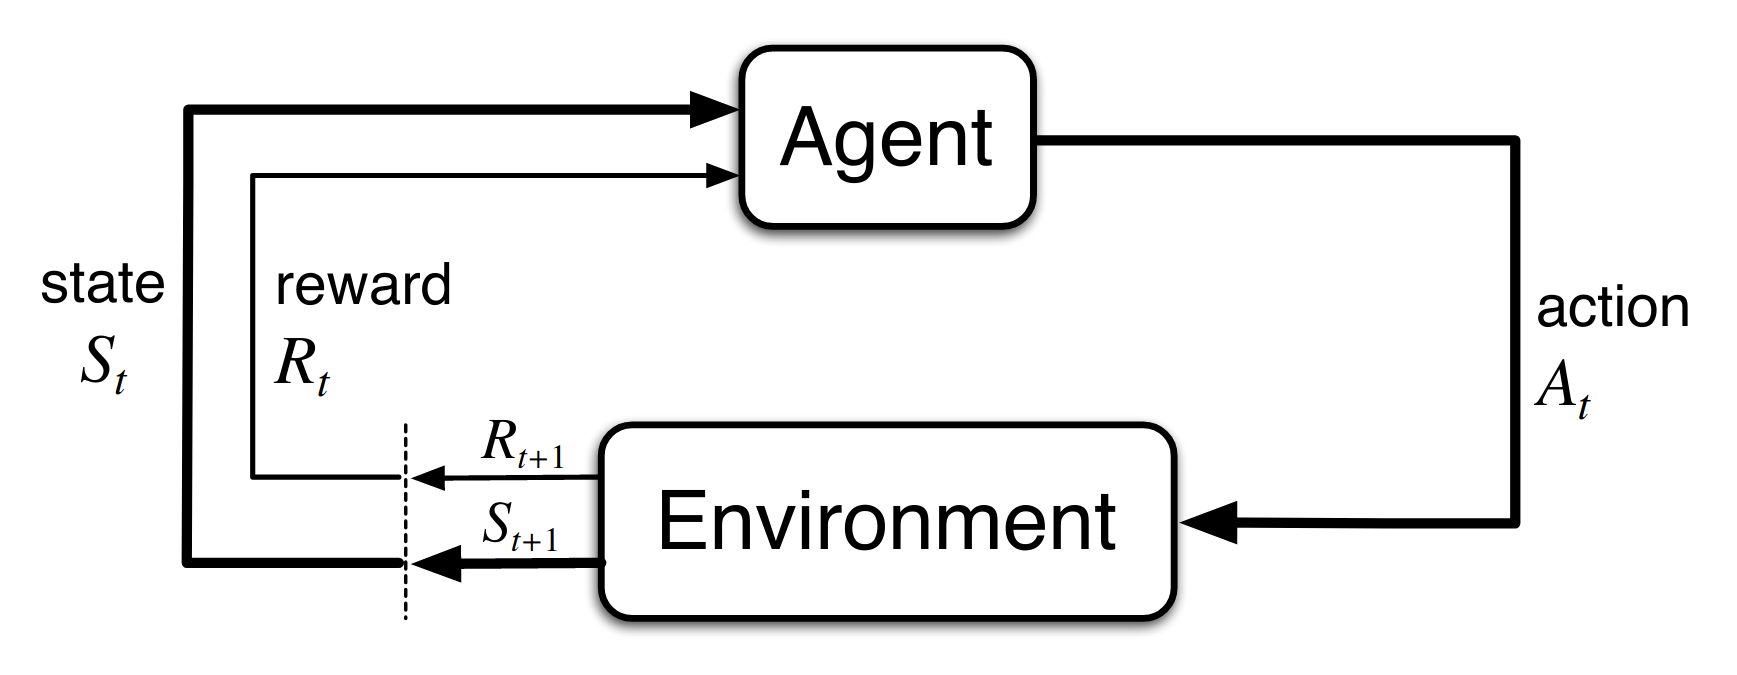
\includegraphics[width=0.8\textwidth]{figures/rl/agent_env_interface}
	\caption{agent environment interaction \cite{SB_all}}
	\label{fig_rl_gen}
\end{figure}

All signals in this model are time dependent. 
Such a model satisfies the Markov Property if next $s'$ and reward $r$ only depend on the current action-state tuple $(s, a)$. If assuming finite state and action spaces together with the Markov Property gives a Finite Markov Decision Process. The environment dynamics can therefore be represented by the bivariate probability distribution
\begin{align}
	p(s', r|s, a) = Pr\{r_{t+1}=r, s_{t+1} = s' | s_t=s, a_t=a\}
\end{align}
Further, if $a_t$ is sampled from $\pi(a_t|s_t)$ the Markov Property induces conditional independence of $(s_{t-1}, r_{t-1})$ and $(s_{t+1}, r_{t+1})$ given $s_t$. \\

The agents task is to predict a policy that maximizes the expected future rewards. This objective is given by
\begin{align}
	\argmax_{\pi}\mathop{\mathbb{E}}_{p_{\pi}}\left[\sum_{t=0}^T r_t | s_0\right]
\end{align}
Here T marks the time limit of the process and $p_{\pi}$ represents the environment dynamics following a action history sampled from $\pi$.\\

\subsection{Value functions}
Most methods of solving eq. (1.2) use so estimations of so called value functions. This are functions that provide a quality measure for an agent evaluating a state-action tuple. \\
Commonly three value functions are used. The state-value function, the action-value function and the advantage-value function. They all depend on the expected discounted future rewards
\begin{align}
	g_t = \sum^{T-t-1}_{k=0} \gamma^k r_{t+k+1} .
\end{align}
Here $\gamma$ is referred to as the discount factor. Its value usually determines how prospective future rewards are weighted in the value function. E.g if $\gamma<1$ rewards that are closer to $t$ get a higher weight than those that are occuring at a later time. For $\gamma>1$ the contrary holds.\\
The state-value function is defined by
\begin{align}
	V_{\pi}(s) = \mathop{\mathbb{E}}_{p_{\pi}}\left[g_t|s_t=s \right]\text{,}
\end{align}
the action-value by
\begin{align}
	Q_{\pi}(s, a) = \mathop{\mathbb{E}}_{p_{\pi}}\left[g_t|s_t=s, a_t=a \right]
\end{align}
and finally the advantage-value by
\begin{align}
	A_{\pi}(s, a) = Q_{\pi}(s, a) - V_{\pi}(s)
\end{align}
it follows
\begin{align}
	V_{\pi}(s) = \mathop{\mathbb{E}}_{a\sim\pi}\left[ Q_{\pi}(s, a)\right]
\end{align}

\noindent Usually the objective is to maximize either one or both of the value functions.
Note that, $\max_{\pi}V_{\pi}(s)$ and $\max_{\pi}Q_{\pi}(s, a)$ satisfy Bellman's principle of optimality. Hence they can be solved exactly by Dynamic Programming. This is referred to as the tabular solution. However for most problems this is not feasible and the value functions are approximated by neural networks. \\

\subsection{Q-learning}
Q-learning is a method to find the action-value maximizing policy by using temporal differences. This often the backbone of policy gradient algorithms. Let
\begin{align}
\pi(\cdot|s) = \softmax_{a}Q_{\pi}(s, a)
\end{align}
then the objective is to approximate $Q_{\pi}$ which is achieved by the temporal difference loss
\begin{align}
\mathcal{L}_{TD} = \frac{1}{2} \left(r_{t+1} + \gamma \max_{a}Q_{\pi}(s_{t+1}, a) - Q_{\pi}(s_t, a_t)\right)^2
\end{align}
this kind of approximation is usually referred to as one step TD method. The optimality follows directly and the convergence of the approximation under certain conditions has been proven in \cite{SBQL}.\\
In contrast to one step TD methods there are Monte Carlo methods which collect the loss over whole episodes where one episode is defined by the history of temporal differences between a starting state and an end state. This methods are often solved by eligibility traces \cite{SBeligibility}. \\
Optimizing eq (1.8) is referred to as on-policy policy optimization where the target policy $\pi$ is the policy which is used when actions are sampled. This however is problematic as the target policy is defined by eq (1.7) depending on $q_{\pi}$ which is not trustworthy as this is the function that is to be approximated. In order to have more control over the sampling of actions which is usually referred to as exploration a data collection policy $\mu(a|s)$ is used. Therefore in an off-policy setting eq (1.8) becomes
\begin{align}
\mathcal{L}_{TD} = \frac{1}{2} \left(r_{t+1} + \gamma \max_{a}Q_{\mu}(s_{t+1}, a) - Q_{\mu}(s_t, a_t)\right)^2\text{.}
\end{align}
and during inference 
\begin{align}
\bar{\pi}(\cdot|s) = \softmax_{a}Q_{\mu}(s, a)
\end{align}
is used. There are many solutions to overcome the distribution mismatch between $\pi$ and $\mu$. Many use importance sampling or variance reduction techniques.\cite{liu2018breaking}

\subsection{Policy gradient methods}

This class of methods optimizes the parameters $\theta$ that define the statistics of a policy $\pi_\theta(a|s)$. Let 
\begin{align}
\rho(\pi) = \sum_{t=1}^{\infty}\mathop{\mathbb{E}}_{\substack{s\sim d_\pi(s) \\ a\sim \pi(a|s)}} \left[ r_t|s_0 \right]
\end{align}
be the expected, discounted future reward per step and let
\begin{align}
d_\pi(s) = \sum_{t=0}^\infty \gamma^t Pr\left\{s_t=s|s_0, \pi\right\}
\end{align}
be the discounted stationary distribution of states under $\pi$. Then
\begin{align}
\frac{\partial\rho_\pi}{\partial\theta} = \sum_s d_\pi(s)\sum_a \frac{\partial\pi(a|s)}{\partial\theta} \bar{Q}_\pi(s,a)
\end{align}
Is the policy gradient with which gradient ascent on the policy can be performed in order to maximize $\rho$. A proof and a thorough discussion can be found in \cite{PGBS}. Note that the policy gradient is on-policy and that $\bar{Q}_\pi$ is an approximation of $Q_\pi$.\\
Since $\pi$ is a probability distribution it follows $\sum_a\frac{\partial\pi(a|s)}{\partial\theta}=0, \forall s \in S$. Therefore
\begin{align}
\frac{\partial\rho_\pi}{\partial\theta} = \sum_s d_\pi(s)\sum_a \frac{\partial\pi(a|s)}{\partial\theta}\left[ \bar{Q}_\pi(s,a)+b(s)\right],\text{\hspace{12mm}} b:S\rightarrow \mathop{\mathbb{R}}
\end{align}
the function $b$ is called a baseline and is often used to reduce variance and bias of the gradient ascent update step. Using $\frac{\nabla_\theta\pi(a|s)}{\pi(a|s)} = \nabla_\theta ln(\pi(a|s))$ and $\mathop{\mathbb{E}}_{x\sim p(x)}[f(x)] = \sum_{x}p(x)f(x)$, rewriting eq (1.13) yields
\begin{align}
\frac{\partial\rho_\pi}{\partial\theta} = \mathop{\mathbb{E}}_{\substack{s\sim d_\pi(s) \\ a\sim \pi(a|s)}}\left[ \nabla_\theta ln (\pi(a|s))\left[ \bar{Q}_\pi(s,a)+b(s)\right]\right]
\end{align}
In practice where there are large state and action spaces the expectations w.r.t $s$ and $a$ become infeasible to obtain. Using $\mathop{\mathbb{E}}_{x\sim p(x)}[f(x)] = \frac{1}{n}\sum_{n}f(x), n\rightarrow\infty, x\sim p(x)$ , ample based learning uses enough samples of $s$ and $a$ in order to obtain a good enough approximation of the expectations. Therefore eq. (1.15) becomes

\begin{align}
\frac{\partial\rho_\pi}{\partial\theta} = \frac{1}{n}\sum_{n} \nabla_\theta ln (\pi(a|s))\left( \bar{Q}_\pi(s,a)+b(s)\right),\text{\hspace{8mm}} s\sim d_\pi(s), \text{\hspace{4mm}} a\sim \pi(a|s), \text{\hspace{4mm}} n\rightarrow\infty
\end{align}

This leads to Actor Critic methods (A2C) where there are two instances that are updated in a turn based fashion. The critic is the value-function approximation and the actor is approximating the policy. Intuitively the critic evaluates the action taken by the actor who uses this evaluation to scale its gradient update (this is the role of $\bar{q}_\pi$ in eq (1.13)).

\subsection{Maximum Entropy Reinforcement Learning}
In off-policy settings it is common to use a data collection policy $\mu$ which has a large entropy in order to encourage exploration of the action and state spaces. The principle of maximum causal entropy has been introduced by \cite{AAAIziebert} and has been elaborated on among others by \cite{DBLP:journals/corr/HaarnojaTAL17}. The key idea is to incorporate an entropy term into the objective function acting like a regularizer. 

\begin{align}
\rho^{\mathcal{H}}(\pi) = \sum_{t=1}^{\infty}\mathop{\mathbb{E}}_{\substack{s_t \sim d_\pi(s_t) \\ a_t \sim \pi(a_t|s_t)}} \left[ r_t + \alpha(t) \mathcal{H}(\pi(\cdot | s_t))|s_0 \right]
\end{align}
Here $\alpha$ is a non-negative regularization weight which is usually monotonically decreasing with increasing $t$ and $\mathcal{H}$ is some entropy measure. If $\alpha$ becomes $0$ eq. (1.17) becomes equal to eq. (1.11), therefore, intuitively $\alpha$ should be high in the early phase of training the policy and the value function and converge to $0$ as the policy gets closer to the perfect policy and therefore can afford to have more certainty in its prediction.
This objective is on-policy and still gives control over the exploration behavior. Usually it does not bother if the policy has high entropy, since during inference the action where "\pi" has maximum probability is selected. This makes especially unimodal distributions attractive. They fixate on single actions and they imply few parameters only that need to be learned (e.g. mean and variance of normal distributions). However often more expressive multimodal distributions fit the true distribution which is approximated better. 
In \cite{DBLP:journals/corr/abs-1906-02771} this idea has been extended by using  normalizing flows. Normalizing flows \cite{papamakarios2019normalizing} are based on the idea of transforming a probability density function by letting each sample undergo a transformation. If this transformation is a diffeomorphism the probability of the transformed sample can be determined. Let $T$ be a diffeomorphism of a real vector $u$ sampled from $p_u(u)$.

\begin{align}
	x=T(u) \text{\hspace{5mm}where\hspace{5mm}} u\sim p_u(u)
\end{align}
then
\begin{align}
p_x(x)=p_u(T^{-1}(u)) |detJ_T(u)|^{-1}
\end{align}
where $J_T(u)$ is the Jacobian matrix of $T$ w.r.t. $u$. I practice an invertible neural network can be trained to transform a simplistic density function into a more expressive one.\\
E.g. let the agent predict mean and variance of a Normal distribution. Actions are the in the data collection process sampled from a transformed Normal distribution where the transform encourages entropy and maybe also multiple modes. Assuming the sampling happened using reparametrization the log probabilities and their gradient in eq (1.14) can still be calculated. This is a on-policy training with a expressive density function and the advantage is that easy reparameterization tricks can still be used since the sampling itself is happening from the base distribution.

\subsection{Soft Actor-Critic (SAC)}
This algorithm was introduced by \cite{haarnoja2018soft}. They aim to maximize the objective in eq. (1.17). Particularly they focus on the selection of the weight factor $\alpha$ and show, that it can be seen as a learnable parameter which is trained jointly with actor and critic networks.\\
SAC is derived from the soft policy iteration where the temporal difference equation for the action value depends on the soft value function which is
\begin{align}
	V_{\pi}(s_t) = \mathop{\mathbb{E}}_{a \sim \pi(a|s_t)} \left[ Q_{\pi}(s_t, a) - \alpha log( \pi(a|s_t)) \right]
\end{align}
the negative log probabilities are the entropy measure in eq. (1.18). The action value function loss yields
\begin{align}
	\mathcal{L}_{critic} = \frac{1}{2}(Q_{\pi}(s_t, a_t) - (\gamma \mathop{\mathbb{E}}_{s_{t+1} \sim d_{\pi}(s)} \left[ V_{\pi}(s_{t+1})\right] + r_t)) ^ 2
\end{align}

For the policy improvement step the policy is updated such that it approximates $\softmax_a(\frac{1}{\alpha}Q_{\pi}(s, a))$ where $Q_{\pi}$ is the soft action value function, learned by minimizing eq (1.21). The loss for the policy then yields

\begin{align}
\mathcal{L}_{actor} = DKL_{a}\left[ \pi(a| s_t) \bigg|\bigg| \frac{exp(\frac{1}{\alpha} Q_{\pi}(s_t, a))}{Z(s_t)} \right]
\end{align}

here, $DKL_{a}$ is the Kullback Leibler Divergence over the actions. $Z(s_t)$ is the partition function of the distribution. 

\begin{align}
	Z(s_t) = \sum_a Q_{\pi} (s_t, a)
\end{align}

It is usually too expensive to evaluate $Z(s_t)$ since it involves integrating/summing over the action value space which means many forward passes through the neural network that represents $Q_{\pi}$. Since $\mathcal{L}_{actor}$ is minimized by gradient descent methods only the gradient is needed. If one expands the KL-divergence term, $Z(s_t)$ becomes additive and therefore vanishes once the gradient is obtained.\\
Note that $\alpha$ gives control over the differences between action values and therefore over the entropy of the resulting distributution. \emph{lemma 2} in \cite{haarnoja2018soft} claims the improvement of $Q_{\pi}$ with each optimization step of $\mathcal{L}_{actor}$.\\
The gradient of eq. (1.23) w.r.t. the parameters $\theta$ of $\pi$ yields

\begin{align}
\nabla_\theta \mathcal{L}_{actor} = \nabla_\theta \mathop{\mathbb{E}}_{\substack{s_t \sim d_\pi(s_t) \\ a_t \sim \pi(a_t|s_t)}} \left[ \alpha log(\pi(a_t|s_t)) - Q_\pi(s_t, a_t) \right]
\end{align}

approximating eq. (1.24) by a sample based method yields

\begin{align}
\nabla_\theta \bar{\mathcal{L}}_{actor} = \nabla_\theta \left[ \alpha log(\pi(a_t|s_t)) - Q_\pi(s_t, a_t) \right]
\end{align}

minimizing this loss by a gradient descent method involves backpropping through a sampling procedure. This can be made differentiable by the reparameterization trick \cite{kingma2013autoencoding}.

\cite{haarnoja2018soft} also provides a method to determine the entropy adjustment $\alpha$ such that it takes the minimal value needed to maximize the maximum entropy objective eq. (1.17) assuming a fixed policy $\pi$.

In practice, reinforcement learning problems have high dimensional action spaces but only one dimensional rewards. Therefore the learned action value function of the critic is also one dimensional in contrast to the actor who predicts the statistics of the policiy for each action dimension. Then the joint probability is the product of probabilities over all actions. This results in summing the log probabilities in eq. (1.25)

\subsection{Common optimization methods}
There are numerous optimization methods for reinforcement learning problems. This is just a listing of only very few but important ones, reviewed and tested in \cite{hessel2017rainbow}.

\begin{itemize}
	\item \textbf{Double Q-learning} \cite{DBLP:journals/corr/HasseltGS15} Conventional Q-learning is affected by an overestimation bias of action values. Decoupling the action selection from its evaluation by learning two action value networks independently resulting in the loss
	
	\begin{align}
		\mathcal{L}_{TD} = \frac{1}{2} \left(r_{t+1} + \gamma Q_{\pi}^{(\bar{\phi})} \left( s_{t+1}, \argmax_{a}Q_{\pi}^{(\phi)}(s_{t+1}, a) \right) - Q_{\pi}^{(\phi)}(s_t, a_t)\right)^2\text{.}
	\end{align}
	Here $\phi$ and $\bar{\phi}$ are the parameters of the independently trained action value functions respectively. A similar method trains two action value functions independently and and takes for all evaluations the min value of the two network predictions. Both methods show a reduction in overestimation as shown in \cite{DBLP:journals/corr/HasseltGS15}.
	
	\item \textbf{Prioritized replay} During data collection, the tuples $(s_t, a_t, r_{t+1}, s_{t+1})$ are stored in a replay buffer and during training phases then sampled uniformly from the buffer. In \cite{schaul2015prioritized} the sampling is not uniform but rather with a probability $p_t$ relative to the last encountered loss of that replay tuple.
	\begin{align}
		p_t \propto \mathcal{L}_{TD} ^ \omega \text{.}
	\end{align}
	Raising the loss to the power of the parameter $\omega$ determines the shape of the distribution. New transitions that did not produce a loss yet are always sampled with maximum priority.
	
	\item \textbf{Multi-step learning} Q-learning bootstraps from single step temporal difference losses. \cite{SBQL} introduced multi-step temporal differences which is the transition from Monte Carlo methods to single step temporal difference methods. The $n$-step return is defined as 
	
	\begin{align}
		r_t^{(n)} \equiv \sum_{k=0}^{n-1} \gamma_t^{k} r_{t+k+1}
	\end{align}
	
	then the multi step TD loss yields,
	
	\begin{align}
		\mathcal{L}_{TD} = \frac{1}{2} \left(r_{t+1}^{(n)} + \gamma^{n} \max_{a}Q_{\pi}(s_{t+n}, a) - Q_{\pi}(s_t, a_t)\right)^2
	\end{align}
	
	optimizing multistep TD losses with $n$ sampled uniformly from the interval $[1..T]$ results in faster learning as shown in \cite{SBQL}.
	
	\item \textbf{Dueling networks} This is an optimization method based on the neural network atrchitecture of value functions in value based RL and was introduced by \cite{DBLP:journals/corr/WangFL15}. It features one state-value and one advantage-value stream of computation that both share a common state feature extractor network $f(s)$. This leads to this factorization of action-values
	\begin{align}
		Q_{\pi}^{(\phi)}(s, a) = V_{\pi}^{(\eta)}(f^{(\xi)}(s)) + A_{\pi}^{(\psi)}(f^{(\xi)}(s), a) - \frac{\sum_{a'} A_{\pi}^{(\psi)}(f^{(\xi)}(s), a')}{N_{actions}}
	\end{align}
	
	Here $\eta, \psi$ and $\xi$ are the parameters of the state-value function, the advantage-value function and the state feature extractor respectively. $\phi$ is the concatenation of $\eta, \psi$ and $\xi$.\\
	The last term in eq. (1.31) approximates $\mathop{\mathbb{E}}_{a' \sim \pi} A_{\pi}^{(\psi)}(f^{(\xi)}(s), a')=0$, this equality follows from combining eq (1.6) and eq(1.7). Then eq. (1.31) follows from eq (1.4), eq (1.5) and eq (1.6).\\
	This method outperforms vanilla, value based RL methods on common RL benchmarks. 
	
\end{itemize}


\section{Geometric deep learning}~\label{sec:gcn}
\noindent Convolutional neural networks use the convolution operation to "filter" a regular grid graph of certain dimension with a filter consisting of learnable parameters. Graph convolution, as introduced by \cite{bruna2013spectral} generalizes this notion of convolutional filtering to arbitrary graphs. Through that it is possible to learn functions on non eucledian, structured domains that have a notion of locality.\\
Since then the field developed rapidly, \cite{Bronstein_2017} provides a good overview of the research that was done so far.\\
Most of the research focuses on the application where graphs are constructed from discretizations of 2-dimensional manifolds, embedded in a 3-dimensional eucledian space, usually called point clouds. However the principle can be used for arbitrary graphs that contain features in their nodes.\\
Typically there are two equivalent definitions of convolution on graphs. One is the spectral definition which suffers from large complexity in terms of memory and time. The other one is a spatial construction motivated from signal flows on graphs which is much faster as it operates with sparse representations of the graph. A quick summary of the latter as in \cite{gilmer2017neural} is given below. \\

Let a graph be represented by $G=(X, (A, E))$ where $X\in \mathbb{R}^{N\times m}$ is a node feature matrix of $N$, $m$-dimensional node feature vectors, with nodes ecoded as $i \in[1..N]$. $A$ is a set of adjacency tuples where $A\in \mathbb{N}^{2\times |E|}$ encodes the set of $|E|$ edges with $n$-dimensional edge features $E \in \mathbb{R}^{|E|\times n}$.

The generalization of the convolutional operator, locally expressed by means of the neighborhood $\mathcal{N}(i)$ around node $i$, is

\begin{align}
	\vec{x}_i^\prime = \gamma \left(\vec{x}_i, \aggr_{j \in \mathcal{N}(i)}  \phi \left(\vec{x}_i, \vec{x}_i, \vec{e}_{ij} \right) \right)
\end{align}

where $\aggr$ is a differentiable and permutation invariant function such as the sum or the mean. $\gamma$ and $\phi$ are differentiable functions represented by multi layer perceptrons. This convolution is also referred to as message passing scheme. All this convolution operations w.r.t. to each node in the graph allow parallel computation what makes this schemes fast.




\section{Mutex watershed}~\label{sec:mtx_wtsd}
The Mutex Watershed algortihm introduced in \cite{wolf2019mutex} is a image partitioning algorithm based on watersheding that is able to operate without a prior seeding.\\
Like most image partitioning algorithms it is defined on a graph $G=(V, E^+ \cup E^-, W^+ \cup W^-)$ with a set of vertices $V$, a set of edges as the disjoint union of attractive edges $E^+$ and repulsive edges $E^-$ and a set of corresponding edge weights $ W^+ \cup W^-$. Each vertex in this graph represents uniquely a pixel in the corresponding image. The edge weights are based on the affinity between the incidental vertices of the respective edge. The affinity between two nodes $i$ and $j$ is the probability $p_{ij}$ of the nodes belonging to the same partition in the posterior partitioning. These affinities can be based on differences in pixel intesities or be predicted by e.g. a CNN. \\
Attractive edges $e_{ij}^+ \in E$ have edge weights $w_{ij}^+ \in W$ with $w_{ij}^+ = p_{ij}$. Repulsive edges $e_{ij}^- \in E$ have edge weights $w_{ij}^- \in W$ with $w_{ij}^- = 1-p_{ij}$. \\
A partitioning on $G$ is defined by the disjoint union of a set of attracive and a set of repulsive edges by the active set $A=A^+ \cup A^-$ that encode hard merges and mutual exclusions of vertices.\\
To represent a valid partitioning, the set $A$ has to satisfy cycle constraints. Defining the set $\mathcal{C}_i(A)$  with $A\subseteq E$ as the set of all cycles in $A$ with exactly $i$ active repulsive edges
\begin{align}
	\mathcal{C}_i(A) := \left\{ c \in cycles(G) \vert c \subseteq A \text{  and  } |c \cap E^- | = i \right\},
\end{align}
a valid partitioning can only be inferred from an active set $A$ if $\mathcal{C}_1(A) = \emptyset $. If additionally $\mathcal{C}_0(A) = \emptyset $, the algorithm can be defined as the search for the minimal spanning tree in each partition.\\
\vspace{8mm}\\
\begin{algorithm}[H]
	\KwData{weighted graph $G=(V, E^+ \cup E^-, W^+ \cup W^-)$}
	\KwResult{clusters defined by spanning forest $A^\star \cap E^+$}
	Initialization: $A = \emptyset$\;
	\For{$(i, j) = e \in(E^+ \cup E^-)$ in descending order of $W^+ \cup W^-$}{
		\If{$\mathcal{C}_0(A \cup \{ e \}) = \emptyset$ and  $\mathcal{C}_1(A \cup \{ e \}) = \emptyset$}{
			$A \leftarrow A \cup e$ \;
		}
	}
	$A^\star \leftarrow A$ \;
	\Return $A^\star$
	\caption{Mutex Watershed \cite{wolf2019mutex}}
	\label{algo:mtx_wtsd}
\end{algorithm}
\vspace{8mm}

An example walk through of the algorithm is depicted in figure \ref{fig_mtxwtsd1}. \\

\begin{figure}
	\centering
	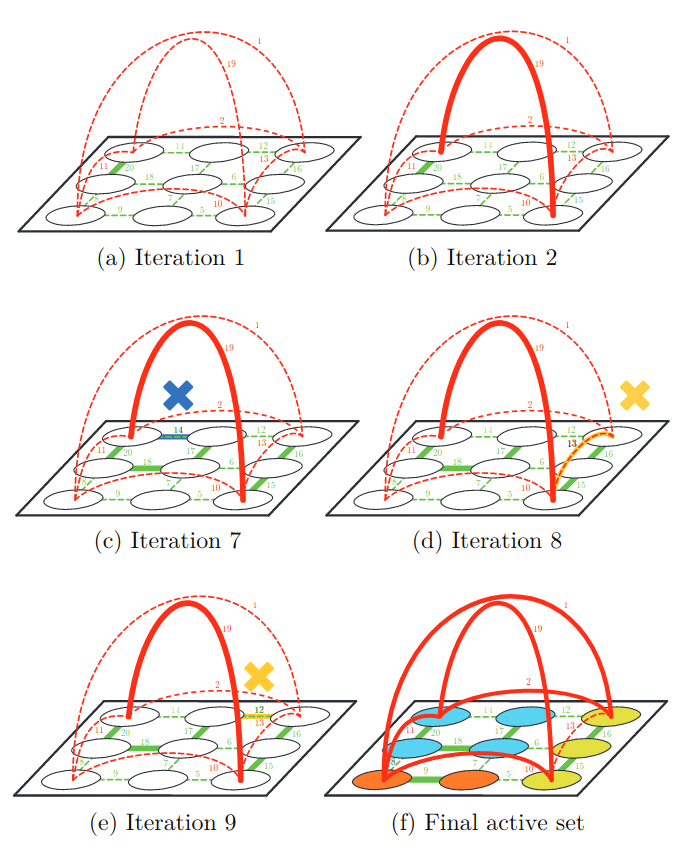
\includegraphics[width=0.5\textwidth]{figures/mutexwatershed/walkthrough}
	\caption{\cite{wolf2019mutex} Some iterations of algorithm \ref{algo:mtx_wtsd} applied to a graph with weighted attractive edges (green) and repulsive (red) edges. Edges that are part of the active set $A$ at each iteration are shown in bold. On termination (f), the connected components in $A \cap E^+$ represent the partitions of the final partitioning. Edges that are not added to $A$ because of the violation of $\mathcal{C}_0$ or $\mathcal{C}_1$ are highlighted in blue and yellow respectively.}
	\label{fig_mtxwtsd1}
\end{figure}

\newpage
Algorithm \ref{algo:mtx_wtsd} minimizes an energy functional that is defined by the active set $A$. This requires the following definition:
\begin{defn}
	\textbf{Dominant power} \cite{wolf2019mutex}: \\
	Let $G = (V, E, W)$ be an edge weighted graph, with unique edge weights $w_e \in \mathbb{R}_0^+$, $\forall e \in E$. Then $p \in \mathbb{R}^+$ is called a dominant power if:\\
	\begin{align}
		w_e^p > \sum_{\substack{t \in E \\ w_t < w_e}} w_t^p \text{\hspace{8mm},} \forall e \in E
	\end{align}
\end{defn}
 This allows the definition of the objective that is solved by algorithm \ref{algo:mtx_wtsd}
 
 \begin{defn}
 	\textbf{Mutex Watershed Objective} \cite{wolf2019mutex}: \\
 	Let $G = (V, E, W)$ be an edge weighted graph, with unique edge weights $w_e \in \mathbb{R}_0^+$, $\forall e \in E$ and $p \in \mathbb{R}^+$ a dominant power. Then the Mutex Watershed Objective is devined as the integer linear program:\\
 	\begin{align}
 		\min_{a\in {0,1}^{|E|}} - \sum_{e \in E} a_e w_e^p \\
		\text{s.t. \hspace{2mm}} \mathcal{C}_0(A) = \mathcal{C}_1(A) = \emptyset \text{, }\\
		\text{with \hspace{2mm}} A := \{ e \in E|a_e = 1 \}
 	\end{align}
 \end{defn}

\section{Image partitioning by multicuts}~\label{sec:multicut}
The multicut problem is a graph cuts problem that is in \cite{10.1007/978-3-642-23094-3_3} redefined for the image partitioning task. The unsupervised partitioning on a grid graph $G=(V, E)$ where each node $v \in V$ corresponds to a pixel in an image can be defined as the following minimization problem

\begin{align}
	\min_{x \in L^{|V|}} \sum_{uv \in E} \beta_{uv} I(x_u \neq x_v) \text{, \hspace{5mm}} L=\{ 1, ..., |V| \}
\end{align}

where $I$ is a indicator function that maps a boolean expression to $1$ if it is true and to $0$ otherwise. $L$ is the set of all possible labels, $\beta_{uv}$ is the edge cost that is active if $u$ has a different label than $v$. $x=(x_v)_{v\in V} \in L^{|V|}$ is a node labeling that defines a partitioning of $V$ into subsets of nodes $S_l$ assigned to class $l$ such that $\bigcup_{l \in L} S_l = V$. Eq. (2.38) defines the unsupervised partitioning problem where the maximum number of classes in the final labeling is the number of nodes $|V|$ in the graph $G$. Therefore the coefficients $\beta$ can depend on the data but are assumed not to depend on prior information about a fixed number of classes $L$. \\
A \emph{multicut} on a graph $G=(V,E)$ with a partitioning $\bigcup_{l \in L} S_l = V$ is defined as 
\begin{align}
	\delta(S_1, ..., S_k) := \left\{ uv \in E | \exists i \neq j : u \in S_i \text{\hspace{1mm}and\hspace{1mm}} v \in S_j \right\}
\end{align}
Where the sets $S_1, ..., S_k$ are called the \emph{shores} of the multicut.
To obtain a polyhedral representation of the set of multicuts on a graph on needs to define incidence vectors $\mathcal{X}(F) \in \mathbb{R}^{|E|}$ for each subset $F \subseteq E$:
\begin{align}
	\mathcal{X}_e(F) = \begin{cases}
	1, \text{\hspace{1mm}if\hspace{1mm}} e \in F \\
	0, \text{\hspace{1mm}if\hspace{1mm}} e \in E \backslash F
	\end{cases}
\end{align}
then the multicut polytope is given by
\begin{align}
	MC(G) := conv\left\{ \mathcal{X}(\delta (S_1, ..., S_k)) | \delta (S_1, ..., S_k) \text{ is a multicut of } G \right\}
\end{align}
and the unsupervised image partitioning problem eq. (2.38) can be written as the equivalent multicut problem

\begin{align}
	\min_{y \in MC(G)} \sum_{uv \in E} \beta_{uv} y_{uv}
\end{align}

defining cycle constraints allows to rewrite eq. (2.42) as the integer linear program (ILP)

\begin{align}
	\min_{y \in [0, 1]^{|E|}} & \sum_{uv \in E} \beta_{uv} y_{uv} \\
	 \text{s.t. \hspace{4mm}} \sum_{uv \in C} y_{uv} & \neq 1 \text{, \hspace{8mm}} \forall \text{ cycles } C \subseteq E 
\end{align}

The cycle constraints in eq. (2.47) enforce that $y$ lies inside the multicut polytope by guaranteeing that there are no active edges inside a shore. There are many solution methods for this problem. The one used in \cite{10.1007/978-3-642-23094-3_3} is based on iteratively solving the ILP in eq. (2.43) without cycle constraints initially, then finding violated constraints in the sense of eq. (2.44), adding them to the ILP and reiterate until there are no more violated cycle constraints.\\
Violated constraints can be found by projecting a obtained solution $y$ to the multicut polytope and checking for differences in the solution and the projection $y'$.
The projection is achieved by assigning a label to each connected component in $G=(V, \left\{ uv | y_{uv} = 0 \right\})$ which produces a valid partition for which the respective \emph{multicut}, and therefore $y'$, can be obtained easily. If there exists an active edge $uv$ inside the solution that is not active within the projection then this is an edge inside a shore and one of the respective violated cycle constraints is obtained by computing the shortest path between $u$ and $v$ inside the shore and adding the active edge $uv$ to that path, yielding a cycle.

\section{Principal component analysis}~\label{sec:pca}
The principal components of a collection of data points can be thought of as the directions in which the variance of the data points is the highest. The magnitude of the variance in the direction of a principal component is referred to as the score of that principal component. All principal component vectors form a orthonormal basis.\\
Consider a data matrix $X \in \mathbb{R}^{n\times p}$ of $n$, $p$-dimensional samples from an arbitrary distribution. The first principal component is

\begin{align}
	w_{(1)} = \argmax_{\norm{w} = 1} \norm{Xw}^2
\end{align}

Since this is a convex optimization problem, the solution can be found by finding the stationary points of the Lagrange function

\begin{align}
	\mathcal{L}(w, \lambda) &= w^TCw - \lambda(w^Tw -1)
\end{align}
where $C = X^TX$. Note that $C$ is hermetian.
The partial derivatives yield	
\begin{align}
	\nabla_w \mathcal{L}(w, \lambda) &= 2Cw-2\lambda w \\
	\nabla_\lambda \mathcal{L}(w, \lambda) &= - (w^Tw -1)
\end{align}

setting eq. (2.47) to $0$ yields

\begin{align}
	0 &= Cw-\lambda w \\
	Cw &= \lambda w
\end{align}

it strikes that eq. (2.50) is an eigenvalue problem. Since $C$ is hermetian its eigenvectors form a orthonormal basis, therefore eq. (2.47) equals to $0$ if $w$ is an eigenvector. To see that the solution to eq. (2.45) is in fact the eigenvector with the largest eigenvalue, one has to substitute eq. (2.50) into eq. (2.46).

\begin{align}
	w^TCw - \lambda(w^Tw -1) = w^TCw = \lambda w^Tw = \lambda.
\end{align}

Since eq. (2.45) is a maximization problem, $\lambda$ has to be the largest eigenvalue.
Therefore the first principal component is the eigenvector $w_{(1)}$ with the largest eigenvalue $\lambda_{(1)}$ of $C$. $\lambda_{(1)}$ is also referred to as the score of the principal component $w_{(1)}$. \\

The remaining principal components are given by the other eigenvectors sorted by their eigenvalues.

\section{Loss functions}~\label{ssec:losses}
This section reviews some important loss functions.

\subsection{Dice loss}\label{ssec:loss_dice}

\subsection{Contrasive loss}\label{ssec:loss_contrastive}

This loss, as defined in \cite{brab2017semantic}, applies to the task of instance segmentation in images. A differentiable function predicts points in a feature space that are embedded in a $n$-dimensional eucledian space. Each predicted point in the embedding space corresponds to a pixel within the image. Ideally the $n$-dimensional embedding vectors for each pixel are close to each other in the embedding space if the corresponding pixels belong to the same instance and distant to each other if not. Then a final clustering algorithm can assign an instance/cluster to each embedding vector.\\
A loss that penalizes wrong predictions can be thought of as a force that pulls pixel embeddings of the same instance together and pushes those of different instances apart.
This loss as defined in eq.(4) in \cite{brab2017semantic} consists of three additive parts. Assuming $C$ is the number of instances in an image (each label id in the ground truth image represents an instance). $N_C$ is the number of elements in cluster $c \in [1..C]$, $x_i$ is a embedding vector where $i$ denotes a pixel. $\mu_c$ the mean embedding of cluster $c$, $\norm{\cdot}$ is the $L1$ or $L2$ distance and $[x]_+ = \max(0, x)$. $\delta_v$ and $\delta_d$ margins that are used to hinge the pull and push forces. That is, the forces are only exerted if the distance that is under consideriation is larger than $\delta_v$ for the intra cluster pulling forces, and smaller than $2\delta_d$ for the inter cluster pushing forces. This allows to learn a more expressive embedding space since the points are allowed to move freely if there are no exerted forces on them.\\

\begin{itemize}
	\item \textbf{variance term} this exerts a intra-cluster pull force that draws pixel embeddings towards the cluster center of their respective instance if the distance to the center is larger than $\delta_v$.
	
	\begin{align}
		\mathcal{L}_{var} = \frac{1}{C} \sum_{c=1}^C \frac{1}{N_c} \sum_{i=1}^{N_c} \left[ \norm{\mu_c - x_i} - \delta_v \right]_+^2
	\end{align}
	
	\item \textbf{distance term} this exerts a inter cluster push force that pushes clusters away from each other by penalozing distances between cluster centers that are smaller than $2\delta_d$.
	
	\begin{align}
		\mathcal{L}_{dist} = \frac{1}{C(C-1)} \sum_{c_A=1}^C \sum_{\substack{c_B=1 \\ c_B \neq c_A}}^C \left[ 2\delta_d - \norm{\mu_{c_A} - \mu_{c_B}} \right]_+^2
	\end{align}
	
	\item \textbf{regularization term} this is a small pull-force that keeps the predicted embedding vectors bounded by pulling them towards the origin.
	
	\begin{align}
		\mathcal{L}_{reg} = \frac{1}{C} \sum_{c=1}^C \norm{\mu_c}
 	\end{align}
\end{itemize}

Then the final loss yields

\begin{align}
	\mathcal{L} = \alpha \mathcal{L}_{var} + \beta \mathcal{L}_{dist} + \gamma \mathcal{L}_{reg}
\end{align}

where $\alpha$, $\beta$ and $\gamma$ are weights for the respective terms.\\

The behaviors of the different terms in the loss are sketched in figure \ref{fig_contrastive}

\begin{figure}[ht]
	\centering
	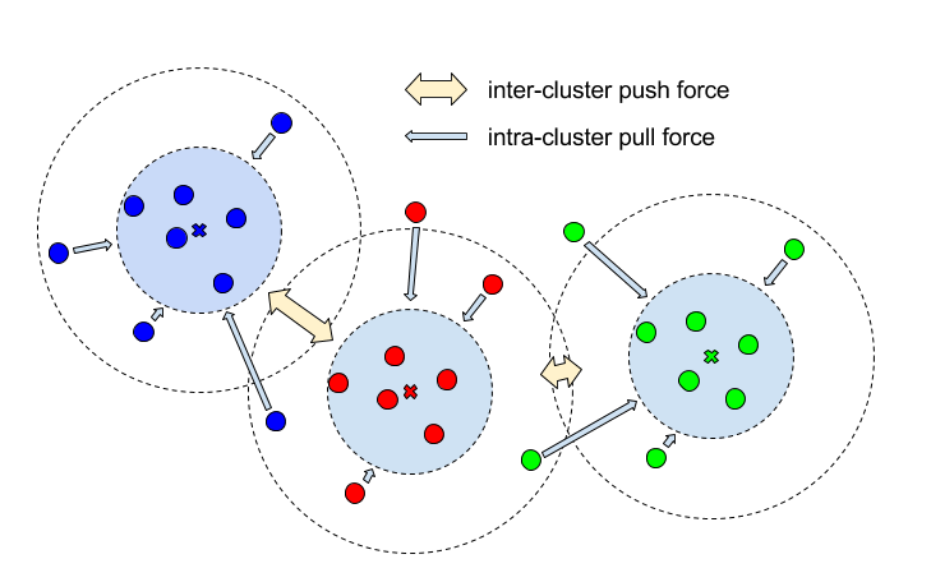
\includegraphics[width=0.5\textwidth]{figures/contrastive_loss.png}
	\caption{As defined by the loss, this are the hinged inter-pulling and intra-pushing forces acting on points in the embedding space \cite{brab2017semantic}}
	\label{fig_contrastive}
\end{figure}

\subsection{Triplet loss}\label{ssec:loss_triplet}
This loss, as defined in \cite{Schroff_2015} is related to the contrastive loss in section \ref{loss_contrastive} in the sense that it is also defined over data points in an embedding space where the resulting embeddings form ideally per instance clusters. The loss function expects three embedding vectors as an input. An anchor $x_i^a$, a embedding that is of the same class $x_i^p$ and one that is of a different class $x_i^n$. Then the loss yields

\begin{align}
	\mathcal{L}_{trpl} = \sum_i^N \left[ \norm{x_i^a - x_i^p}^2 - \norm{x_i^a - x_i^n}^2 + \alpha \right]_+ \text{\hspace{1mm}.}
\end{align} 

Again $[x]_+ = \max(0, x)$, $N$ is the number of all possible triplets $(x_i^a, x_i^p, x_i^n) \in \mathcal{T}$ in the embeddings, $\norm{\cdot}$ is the $L2$ norm and $\alpha$ is a enforced margin between positive and negative pairs. The training behavior using $\mathcal{L}_{trpl}$ as a loss is depicted in figure \ref{fig_triplet}. \\

\begin{figure}[ht!]
	\centering
	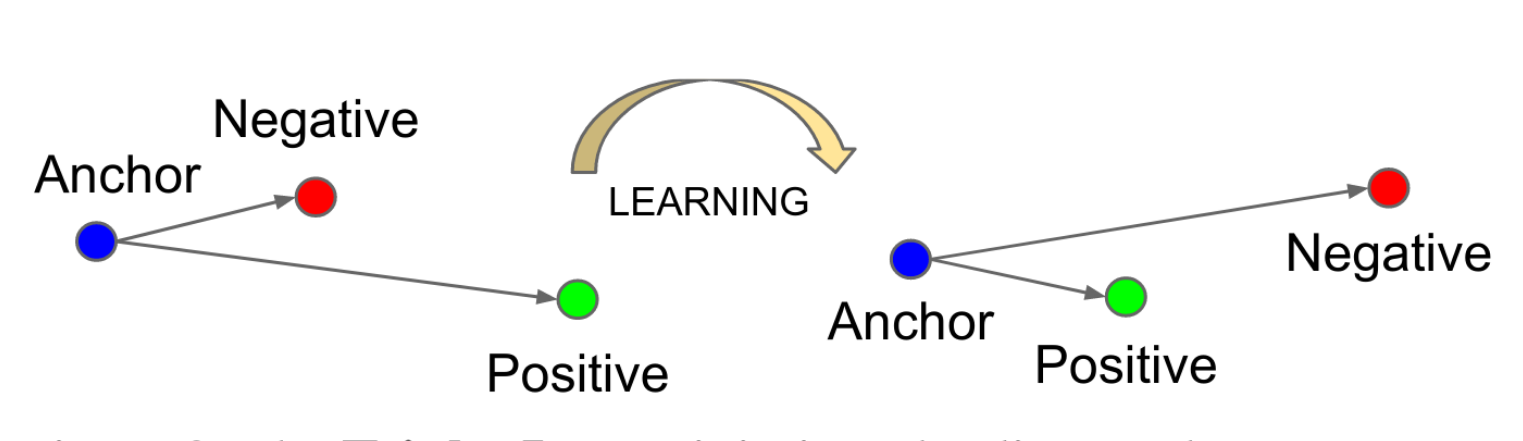
\includegraphics[width=0.5\textwidth]{figures/triplet_loss.png}
	\caption{Position of triplets in the embedding space before and after training \cite{Schroff_2015}}
	\label{fig_triplet}
\end{figure}

Often times $N$ is very large and the loss requires too many resources to calculate. Therefore it is crucial to select triples that are active, namely $\left\{ (x_i^a, x_i^p, x_i^n) \bigg| \left[ \norm{x_i^a - x_i^p}^2 - \norm{x_i^a - x_i^n}^2 + \alpha \right]_+ \neq 0 \right\}$ . However different selection strategies end in very different results regarding training time and convergence to satisfactory optima. E.g. picking only triplets that produce a high loss value can result in a training converging quickly into bad local optima.
To prevent the embeddings from diverging a regularizer term is added in order to constrain the embedding vectors to the unit hypersphere surface.
\begin{align}
	\mathcal{L}_{reg} = \sum_i^M\frac{1}{2}(\norm{x_i} - 1)^2
\end{align}

Here $M$ is the number of pixels in the image. The final loss therefore yields

\begin{align}
\mathcal{L} = \mathcal{L}_{trpl} + \beta \mathcal{L}_{reg}
\end{align}

where $\beta$ is a scalar weight for the regularizer term.
 \pagebreak

\setcounter{figure}{0}
\setcounter{table}{0}
\setcounter{equation}{0}
\chapter{Methods}~\label{chap:rl_for_seg}

\section{Using RL for the image segmentation task}~\label{sec:rl_for_seg}

In this section the task of image segmentation is fit to the RL framework.\\
The agent takes the role of predicting action distributions where sampled actions perform some kind of change to the input of a segmentation algorithm. Rewards can be calculated from the resulting segmentation. The segmentation algorithm would therefore be part of the environment.\\
Common RL problems are usually problems that are easy to evaluate like determining the winner of a board game or evaluating a robots position relative to a target position. Also, often intermediate results are not rewarded at all or given a small negative reward in order to put pressure on the fast arrival at the final state.\\
In RL there is typically a physical environment that can be measured by some sensory devices. This measurements reflect the current state and a reward calculation based on that state can take place. For the task of image segmentation such an environment can not be found or measured.\\
The label predictions would have to be projected from the image plane into the "real world" where measurements could take place. Of course it is not clear how to do that, therefore the reward generation has to be based on a computational model of the environment. A predicted segmentation can only be evaluated if enough information on the objects within the input image is known a priori. E.g number of object instances per object class, position, texture, shape etc..\\
Given such an evaluation and given that the function that is optimized by the agent is capable of capturing the underlying probability distribution of data label pairs, the described RL setting is theoretically able to learn the task of image segmentation in a fully unsupervised way.\\


\section{Using RL for pixel affinity predictions}~\label{sec:rl_for_seg}

This work started with the idea of an RL setting where an agent manipulates affinities between pixel pairs. Those affinities form an input to the Mutex Wateshed algorithm (see section \ref{sec:mtx_wtsd}).\\
The edge set that the Mutex Watershed typically works with are short range attractive edges and long lange repulsive edges where the length of the repulsive edges is dependent on the object sizes in the image. That means that there should be exactly one attractive edge for every directly neighboring pair of pixels and some long range repulsive edges. Defining the problem by manipulating affinities leads to a hard task since there are simply so many.\\
RL methods learns from rewards resulting from actions and an initial state. To achieve convergence, initially there need to be some rewards of a high value, that means that the actions taken lead to a fairly good segmentation. However when starting learning a network from noise it outputs completely arbitrary actions that unlikely lead to a high reward because the action space is simply too large.\\
The RL-typical bootstrapping works only if there is a meaningful gradient in the reward signal, even for random actions. It is not uncommon in RL to have a large action space while the reward is a single scalar value. If it would be possible to calculate more meaningful rewards, say per subregion in the image, one could compute a RL loss term for each of those subregions only considering the actions that manipulated affinities within this region.\\

To downsize a image segmentation problem, it is common to work with superpixels \cite{10.1007/978-3-642-23094-3_3} rather than  with pixels. A superpixel segmentation or oversegmentation is usually achieved by watersheding or smoothing algorithms.
Using Mutex Watershed one can simply globally decrease the edge weights of the attractive edges in order to arrive at an oversegmentation.
Starting from such an oversegmentation and assuming that the ground-truth segmentation is a partitioning of the superpixels, focusing solely on merging and unsmerging superpixels would be sufficient. Concerning the Mutex Watershed algorithm, a merge of two superpixels would be done by turning all the repulsive edges between them into attractive ones and vice versa for unmerging. Therefore one needs a decision/action for every neighboring pair of superpixels.\\
However there are two problems with this, first one can only perform hard merges and unmerges which leads likely to contradictions for example consider 3 adjacent superpixels and there are 2 merges and 1 unmerge predicted. This is of course nothing Mutex Watershed cannot handle but the result is likely to be not a partitioning of the superpixels and therefore not the intended result.\\
The second issue is that for CNNs it is difficult to make predictions on affinities between adjacent superpixels due to the irregularity of the region adjacency graph of the superpixels.
\section{Overview over the proposed pipeline}~\label{seg:ov_pip}

To overcome the two problems stated in the previous section, the following is done. Making hard decisions on merges and unmerges between superpixels is bad because of the arising contradictions where cycle constrains easily become violated but also because a hard thresholding of predictions has to be performed which takes away all the information that lies in the uncertainty of this predictions.\\
Both those issues can be overcome by predicting affinities on the edges between neighboring superpixels which can be transformed into costs and a minimum cost multicut (see section \ref{sec:multicut}) of the superpixel graph can be computed. This leverages the uncertainty of the network predictions and overcomes violated cycle constraints.\\
The second issue that arises from the irregularity of the superpixel graph can be overcome by using a graph neural network (GCNN)that predicts edge weights between superpixels by performing graph convolutions (see section \ref{sec:gcn}). However this generates the problem that there have to be regular representations for superpixels. Of course one solution would be to have two GCNNs, one for intra superpixel convolution and pooling, down to a vector representation of each superpixel and one for inter superpixel convolution using the vector representations. The problem here is the intra superpixel GCNN. Regular graph covolutions on image data makes not a lot of sense because it is not able to capture spatial information like object shapes very good. There are some proposals \cite{monti2016geometric} that introduce spatial dependent features to graph cnvolutions. However considering the power of CNNs with regular images, it makes more sense to use those in favor of GCNNs.\\
Getting superpixel representations from a CNN can be done using a embedding network that predicts pixel embeddings by minimizing a contrastive loss (see section \ref{ssec:loss_contrastive}). Still assuming, that the ground truth segmentation is a partitioning of the superpixels, it is safe to assume similar pixel embeddings in terms of the distance used in the loss for all pixels within a superpixel. Therefore one can average over all pixel embeddings within a superpixel in order to arrive at a vector representation that is used as node features in the following GCNN.\\
The described model is depicted in figure \ref{overview}.


\begin{figure}[ht!]
	\centering
	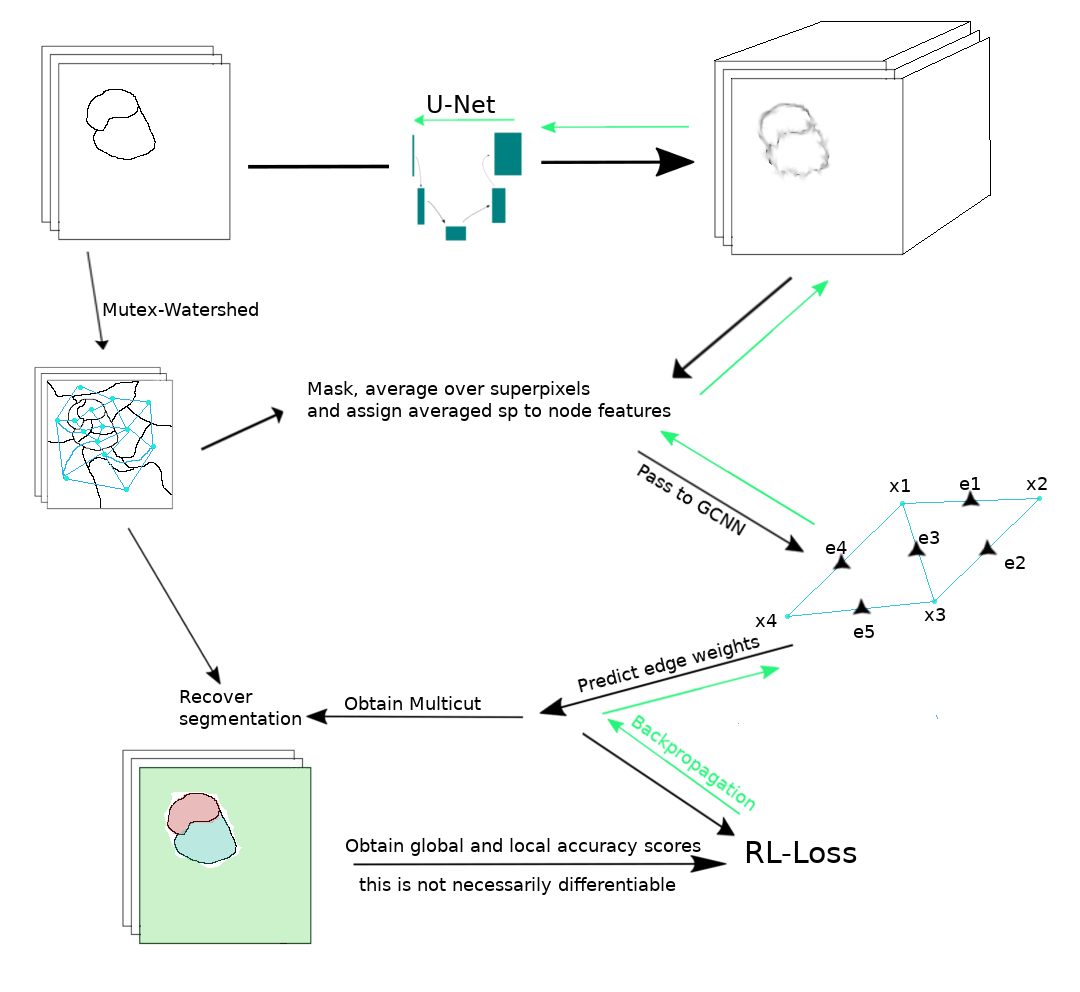
\includegraphics[width=1\textwidth]{figures/images/sketch_overall.png}
	\caption{A rough sketch of the proposed pipeline. Starting from raw data (top left), a superpixel graph is obtained with the Mutex Watershed algorithm \ref{algo:mtx_wtsd} and pixel embeddings (top right) are obtained with an embedding network. With node features computed as the average pixel embedding per superpixel a GCNN predicts logits on the edges of the superpixel graph. The logits are used to compute chances which in turn are used to compute costs based on which a min cost multicut of the superpixel graph is computed from which a segmentation is obtained. This segmentation is then evaluated and a reward is produced which is then used in the RL loss.}
	\label{overview}
\end{figure}


The following sections go into detail of every part in the sketch in figure \ref{overview}
\section{The pipeline in the RL terminology}~\label{seg:pip_tl_term}

As shown in \ref{fig_rl_gen} in all RL problems there are two main instances acting and sending signals to each other. A closer look at each instance and signal as well as their definition within the context of the task is given below. 

\subsection{The state}
Letting the current state be the concatenation of the raw data, a superpixel segmentation $sp$ of the raw data $rw$ and a final segmentation $seg_t$ that is a partitioning of the superpixels $s_t=\left[ rw, sp, seg_t \right]$. Therefore the only part of the state that is ever updated during training on a single image $rw$ is $seg_t$. That means, the only part of the state space that needs to be explored by the agent is defined by $seg_t$. If the segmentation would not be based on superpixels the number of possible states would be a much higher in constrast to $seg_t$ relating to a superpixel partitioning. The state space is the search space in which only one point correponds to the ground-truth.

\subsection{The actions}
The formulation of the actions depend on the RL algorithm used. There are algorithms for discrete and for continuous action spaces. The predicted target are probabilities for merge affinities, therefore values between 0 and 1. So it would be natural to predict continuous actions between 0 and 1 that can then directly be taken for the target merge affinity.\\
However most algorithms with a policy based on value functions like Q-learning are defined only for discrete actions. Algorithms incorporating policy gradients can usually defined for both discrete and continuous action spaces. When working with discrete actions there are 2 possibilities of their definition. \\
\begin{itemize}
	\item one possibility is to directly predict values for discretisized probabilities. Depending on the degree of discretization this might lead to large complexity. Also this makes it possible to diverge away from an initial state very fast, namely within one step. If there is an initial state which is likely already close to the ground truth this is not favorable.
	\item the other possibility is to predict values for actions that are operating on the current state of edge values. E.g a state action value to add or subtract a fixed scalar $c$. Here the level of discretization depends on the magnitude of $c$ which does not change the memory complexity of the output however it has a direct affect on the number of steps that are neccessary to arrive at a target state. This method also favors a more continuous divergence from an initial state.
\end{itemize}

\subsection{The reward}
The reward is crucial for the whole training behavior. The right modelling of the reward signal principally decides for fast convergence to the target solution and the avoidance of "getting stuck" in local optima.\\
If a set of training image-label pairs is available it makes sense to derive a ground truth value for every edge in the superpixel graph. Then the reward is per edge as the distance of the current edge state to the ground truth edge. This is the most accurate reward that can be obtained. Nevertheless this version comes with the drawback of generating large variance in the updates of the state action value function. The contrast to this would be the prediction of a single state action value. This certainly smoothes out any variance in the single predictions but it is also too coarse when it comes to larger superpixel graphs. This problem is in more detail attendet to in section \ref{blabla}.

\subsection{The agent}
The role of the agent is taken mainly by the embedding network, the GCNN and the optimization of those. Its input is the input to the embedding network which is the current state $s_t$. It outputs statistics of a probability distribution per edge. Depending of the choice of algorithm this can be arrays of probabilities for a categorical probability distribution in the case of discrete actions, or the statistics of a proibability desity fucntion in the case of continuous actions. The latter requires a sigmoid transformation of the samples to guarantee they fit the requirement of being a probability.

\subsection{The environment}
The environment receiving actions $a_t$ that act on a state $s_t$ producing $s_{t+1}$ as well as a reward $r_t$. Therefore it mainly consists of the multicut algorithm updating the state based on the actions and of some evaluation scheme for the new state in order to calculate rewards. This scheme can be based on ground truth segmentations or on prior knowledge or both.

\subsection{The problem of local optima}
Usually the ground truth of edge weights reveils a inbalance in attractive and repulsive edges. Due to the nature of an oversegmentation there are a more attractive edges than repulsive edges. This inbalance generates the local optimum of exclusively attractive edges. RL algorithms are known for converging to local optima and also perturbations of the rewards are not able to prevent this.\\
This kind of local optimum is known in image segmentation problems and has been adressed by many losses like focal loss aor dice loss. The dice score can easily directly be transferred to edge value predictions. The problem here is that this produces a single scalar reward. This is a problem because there can easily be a few hundreds or even thousands of edges within a superpixel graph. Having a scalar reward signal is to vague to infer from to actions on single edge values.\\
Most RL benchmarks incorporate action dimensions that are less than $10$ which is a small enough number to have one global state action value.\\
Transferring this to the prediction of edge values on a graph would be a single state action value per subgraph of roughly size $10$. This has the advantage of training a state action value function globally for the predictions on each subgraph. Therefore, if ground truth is available, one can use the dice score over a subgraph as a reward signal. This smoothes out class inbalances as well as variances of single edge state action values. This method is shown in figure \ref{fig_sg}. The figure also roughly sketches method to compute per subgraph rewards in an unsupervised fashion. The subraphs can and should overlap in order to smooth out variances in the reward signal. Since a GCNN is used for the state action value prediction it makes sense to select subgraphs with a high density which increases the information flow in the graph convolution.

\begin{figure}[ht!]
	\centering
	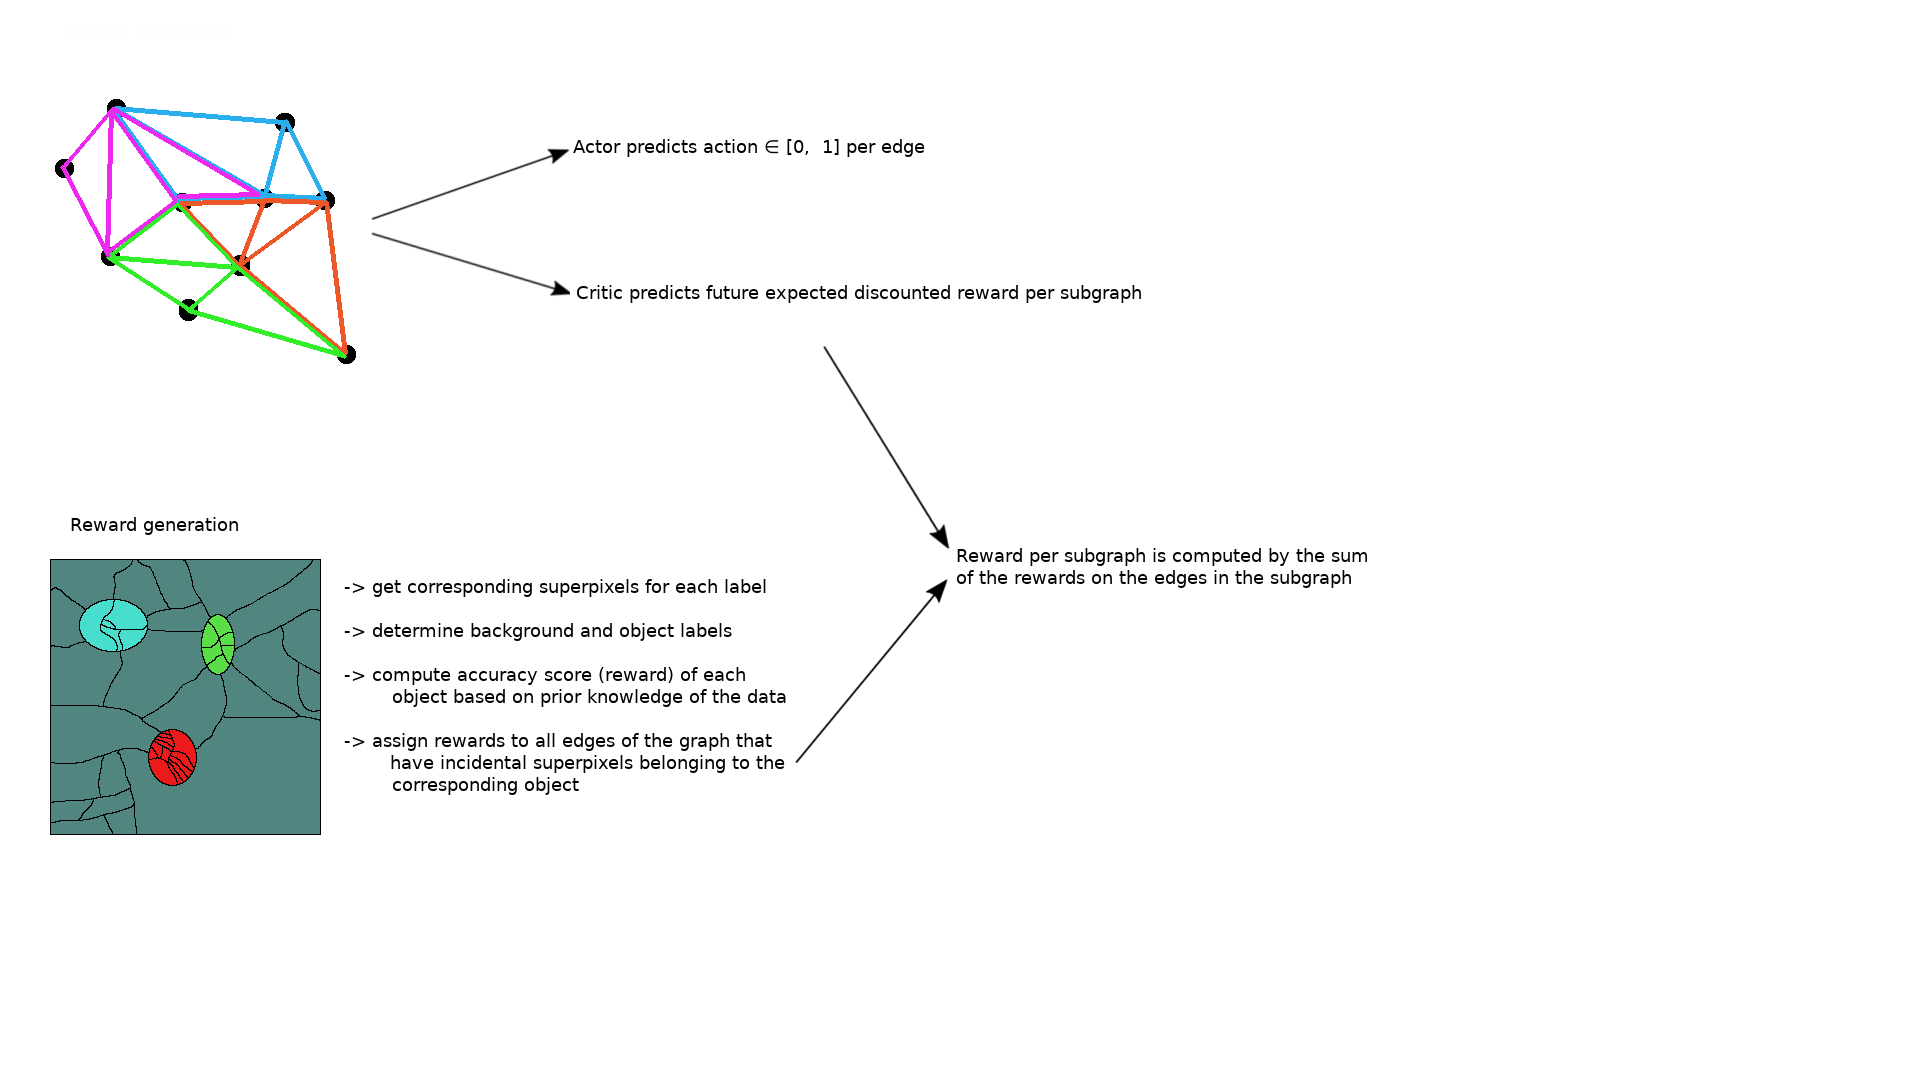
\includegraphics[width=1.5\textwidth]{figures/images/reward_calc_sketch.png}
	\caption{A rough sketch of the reward calcuation on subgraphs with 7 edges and the resulting losses in an actor critic setting}
	\label{overview}
\end{figure}

\subsection{Definition of the RL algorithm}
Vanilla Q-learning or REINFORCE are algorithms that operate in discrete action spaces. The advantages of that have been mentioned. However for the prediction of probabilities it is more natural to use a continuous action space. The drawback is that it is possible to diverge fast from an initial state. Such a divergence can easily be penalized by the reward signal e.g by calculating the distance of current state to the initial state and subtracting that distance from the reward when it surpasses a certain margin. \\
Therefore the selection falls to the SAC algorithm \ref{ssec:sac} which is a confortable choice because it is defined for continuous actions and it takes care of sufficient exploration. 

It is easy to adjust eq. (2.26) in section \ref{ssec:sac} for predictions on subgraphs. Considering a subgraph size of $10$ and selecting the normal distribution for the policy $\pi$. The GCNN predicts for every edge mean $\mu$ and variance $\sigma ^2$ of its action distribution. \\
Drawing a reparameterized \ref{ssec:reparam} sample from the distribution follows a sigmoid transform of the sample. The change of variables formula \ref{ssec:norm_flows} allows for the computation of the probability density of the transformed sample. \\
The joint probability density of all actions per subgraph is given by the product of their respective densities. Therefore eq. (2.26) in section \ref{ssec:sac} is rewritten as

\begin{align}
	\nabla_\theta \bar{\mathcal{L}}_{actor} = \nabla_\theta \sum_{sg \in G} \left[ \alpha \sum_{a_t\in sg}log(\pi(a_t|s_t)) - Q_\pi(s_t, a_t)_{sg} \right]
\end{align}

Here $G$ is the set of sets that contain the respective actions for each subgraph. $Q_\pi(s_t, a_t)$ is a function taking the current state action tuple and maps it to $\mathbb{R}^n$ where $n$ is the number of subgraphs in $s_t$. $Q_\pi(s_t, a_t)_{sg}$ denotes the predicted state action value for subgraph $sg$.\\
eq. (2.22) in section \ref{ssec:sac} does not change considering the rewards are per subgraph as well.\\
Additionally to the optimization techniques within the SAC \ref{ssec:sac} algorithm, prioritized experience replay \ref{ssec:common_opt} is used.\\
RL problems are usually of the form that multiple steps lead to an end state $T$. Since here, directly sampling affinity values from the policy makes it possible to reach any state within one step, it is sufficient to define $T=1$. Stopping after one step has the advantage that the state action function becomes much simpler. The feature to be able to reach any state from any other state makes all parts of the state that are dependent on $t$ redundant. Therefore $s_t$ can be redefined to $s_t=s=[rw, sp]$.\\
Setting $T=1$ the loss in e(2.22) becomes

\begin{align}
	\mathcal{L}_{critic} = \frac{1}{2}(Q_{\pi}(s_t, a_t) - r_t) ^ 2
\end{align}

While this yields a simple action state function to approximate, there is also a point in saying that this definition is not a "real" RL setting anymore. However the RL loss still gives the advantage that the supervision signal (the reward here), does not have to be differentiable, which is the main justification for this pipeline.
\section{Obtaining superpixels from mutex watershed}~\label{seg:pip_mutex}
There are many algorithms that can be used to compute a superpixel segmentation. Mutex Watershed (see section \ref{sec:mtx_wtsd}) is a very flexibly method because it relies on affinities and there are many methods to obtain those, like learned affinities or directly based on pixel intensities.\\
With e.g. a CNN a very generic affinity predictor can be trained. Globally scaling repulsive and/or attractive edge weights allows for control over the granularity of the superpixels. In addition to that, Mutex Watershed is a comparatively fast algorithm under certain conditions that are mainly dependent on the amount of strong repulsive edges.\\
Having the superpixel segmentation, it is straight forward to generate a region adjacency graph from that.

\section{The embedding network}~\label{seg:pip_embed}

The embedding network was realized with a U-Net architecture \cite{ronneberger2015unet} where the final layer outputs 16 channels. There are several ways to train the embedding network. If ground truth is available it can be trained prior to the SAC-training with the contrastive loss \ref{ssec:loss_contrastive}.\\
If there is no ground truth there are three different bootstrapping procedures that can be included to the training of the SAC.\\
\begin{itemize}
 	\item The first one is the optimization of the embedding network through the RL losses. This is possible, because the masking of the embeddings by the superpixels followed by the averaging procedure is differentiable w.r.t. the pixel embeddings. The embedding network forms one common feature extractor for actor and critic. Intuitively it should be more stable if it is optimized only by one of the two loss terms. Since the actor smooths out variances and wrong probabilities in the Gibbs distribution of the critics prediction, the better choice for optimizing the embedding network should be the backpropagated gradient of the actors loss function.
 	\item The second procedure is a mixture of contrastive loss \ref{ssec:loss_contrastive} and triplet loss \ref{ssec:loss_triplet} based on the action predictions of the agent (defined by the mean of the predicted policy). Hereby all pixel embeddings belonging to the same superpixel should be close to each other in the embedding space. This is namely eq. (2.53) in section \ref{ssec:loss_contrastive} where each superpixel corresponds to one cluster.\\
 	For the inter cluster pushing \emph{or} pulling forces, a triplet loss of the form in eq. (2.57) in section \ref{ssec:loss_triplet} is used. The triplets can be found by evaluating the action predictions of the agent.\\
 	A positive superpixel pair is defined by the existence of a path between those superpixels in their region adjacency graph that has only action values on the edges that are below a certain threshold $tl$.\\
 	On the contrary, a negative pair is one that has at least one path between the two superpixels where at least one action value on an involved edge is above a certain threshold $th$.\\
 	Attractive paths between superixels in the region adjacency graph can be found with Dijkstra's algorithm by setting all weights (means of the action distributions) in the weighted adjacency matrix that are above $tl$ to $+\infty$ and then accepting all paths in the result that are not $+\infty$.\\
 	In contrary, repulsive paths between superpixels can be found by setting all weights in the weighted adjacency matrix that are above $th$ to $+\infty$ and accepting all paths in the result that are $+\infty$.\\
 	This selection of triplets does not protect from contradictions in the underlying segmentation. A valid underlying segmentation can be obtained by removing superpixel pairs that violate cycle constraints similar to eq. (2.36) in section \ref{sec:mtx_wtsd}.
 	\item The third method is in its result very similar to the second method, but here the triplet selection is based on the final segmentation $eseg_t$. This method does not suffer from violated cycle constraints and is chosen over the second method. However keep in mind, that this method is based on the sampled actions and not on the mean action of the policy as method two. To get the result based on the expected actions there needs to be an additional run of the Multicut algorithm.
\end{itemize}
The last two methods should happen interchangeably to the SAC training, where the optimization step frequency of the embedding network should be much lower and the loss should be over a "larger" mini batch considering high variances in early SAC predictions.
\section{The actor critic networks}~\label{seg:sag_gcn}

In this section the involved GCNN's are discussed in detail. There is one network predicting the statistics for the policy. This is referred to as the actor network. The implemented graph convolution on a directed graph for $K$ convolution iterations is defined the update functions\\

\begin{align}
\vec{e}_{ij} &= \eta \left( \phi_1 \left(\vec{x}_i, \vec{x}_j \right)\right)\\
\vec{x}_i &= \eta \left( \gamma_1 \left(\vec{x}_i, \frac{1}{deg(\mathcal{N}(i))} \sum_{j \in \mathcal{N}(i)}  \vec{e}_{ij} \right)\right)
\end{align}

For the first iteration as there are no edge features initially, the following iterations are defined by the update functions

\begin{align}
\vec{e}_{ij} &= \eta \left( \phi_k \left(\vec{x}_i, \vec{x}_j, \vec{e}_{ij} \right)\right)\\
\vec{x}_i &= \eta \left( \gamma_k \left(\vec{x}_i, \frac{1}{deg(\mathcal{N}(i))} \sum_{j \in \mathcal{N}(i)}  \vec{e}_{ij} \right) \right)\\
\text{for }k&=1...K-1
\end{align}

Here $\phi_k$ and $\gamma_k$ are multi layer perceptrons and $\eta$ is a elementwise non linear function. $i$ is the node index of the sink node and $j$ the node index of the source node for each edge. The region adjacency graph of the superpixels is undirected therefore it is converted to a directed graph, by swapping each undirected edge for two directed edges, beforehand. The final $K^{\text{th}}$ iteration is defined by the update functions

\begin{align}
\vec{e}_{ij} &= \eta \left( \phi_K \left(\vec{x}_i, \vec{x}_j, \vec{e}_{ij} \right)\right)\\
\end{align}

Where the the number of elements in the output vector $\vec{e}_{ij}$ corresponds to the number of the required scalar values that define the distribution used for the policy. This could be all coefficients of a categorical distribution in a discrete action space setting or mean and variance of a normal distribution in a continuous action space setting.\\

The GCNN's approximating the state action values are referred to as the critic networks. There are two of them of equal architecture but distinct parameters, incorporating Double Q-Learning \ref{text:doublQ}. The first $K$ graph convolutions are equally defined to the actor network with the difference that the last convolution outputs vectors $e_{ij}$ of the same lengths as the input node feature vectors.
Following that, the graph without node features and edge features $e_{ij}$ is split into unconnected subgraphs with a fixed number of $l$ edges. The following iteration on the subgraphs is defined by the update

\begin{align}
\vec{x}_i &= \eta \left( \gamma_1 \left(\vec{x}_i, \frac{1}{deg(\mathcal{N}(i))} \sum_{j \in \mathcal{N}(i)}  \eta \left( \phi_K \left(\vec{x}_i, \vec{x}_j\right)\right) \right)\right)
\end{align}

and the last graph convolution iteration by

\begin{align}
\vec{e}_{ij} &= \eta \left( \phi_K \left(\vec{x}_i, \vec{x}_j \right)\right)
\end{align}

the scalar state action value per subgraph is obtained by

\begin{align}
	\gamma_{Q}\left( \frac{1}{l} \sum_{ij\in sg} e_{ij} \right)
\end{align}

where $\gamma_{Q}$ is a mlp outputting a scalar value.
\section{Finding subgraphs}~\label{seg:sag_gcn}
The selection of subgraphs has the only hard restrictions that all selected subgraphs should consist of $l$ edges and that the union of subgraphs should cover the region adjacency graph of the superpixel segmentation. Additional to that it is encouraged to select overlapping subgraphs and subgraphs of high density. The latter can be rewritten by finding subgraphs with the smallest possible node counts. Also the overlaps should not be too large such that the result is still a feasible number of subgraphs. \\
Finding the densest subgraph of size $l$ in a graph $G=(V,E)$ is in general a NP-hard problem \cite{densestSg}. The implemented algorithm is a fast heuristic that leverages the properties of the region adjacency in $G$ where one can assume a relative even density over the whole graph.\\
The heuristic starts by sampling a random edge $(ij)\in E$, that is not contained in any subgraph so fara, adds it to the new subgraph $SG=(SV,SE)$ and pushes its incidental nodes to a priority queue $pq$ with starting priority value $0$ (smaller value corresponds to higher priority). Nodes are drawn from $pq$ until the respective subgraph has the right amount of edges. Drawing a node $n$ from $pq$ is followed by iteratively verifying if there is a node $m$ s.t. $(nm)\in E$ and $m\in SV$, if yes than $(nm)$ is added to $SG$ and $m$ is added to $pq$ with a priority that is incremented by $1$. If not all to $n$ adjacent nodes where accepted and the corresponding edges added to $SG$, the priority of $n$ is decreased by the amount of edges that where added and pushed into $pq$ again.\\
The next iteration starts by drawing the next node from $pq$. If all elements in $pq$ where drawn without an edge being added to $SG$ and $SG$ being still incomplete, the last drawn nodes $n$ last examined neighbour $m$ is added to $pq$ and  the edge $nm$ is added to $SG$.\\
This is repeated until all subgraphs cover $G$. The worst case of this method would be tree-like subgraphs overlapping completely except for one edge. However for region adjacency graphs this is unlikely too happen and can be ignored.\\
The pseudo code for the described heuristic is given in algorithm \ref{algo:sgs}.\\
\vspace{8mm}\\
\begin{algorithm}[H]
	\KwData{$G=(V, E)$, $l$}
	\KwResult{subgraphs by sets of $l$ edges}
	Initialization:$SG = \emptyset$\;
	\While{$E\backslash SG \neq \emptyset$}{
		pq = PriorityQueue\;
		prio = 0\;
		n\_draws = 0\;
		$sg = \emptyset$\;
		$i, j = (ij)$ s.t. $(ij)\in E\backslash SG$\;
		pq.push($i$,prio)\;
		pq.push($j$, prio)\;
		$sg = sg \cup (ij)$\;
		\While{|sg| < $l$}{
			$n$, n\_prio = pq.pop()\;
			n\_draws ++\;
			prio ++\;
			$adj = \{(nj) | \exists (nj)\in sg\}$\;
			\ForAll{$(nj)\in adj$}{
				pq.push(j, prio)\;
				$sg = sg \cup (nj)$\;
				n\_draws = 0\;
			}
		\uIf{$|adj| < $ deg$(n)$}{
			n\_prio -= $(|adj|-1)$\;
			pq.push($n$, n\_prio)\;
		}
		\uIf{n\_draws = pq.size()}{
			$j \in \left\{j |(nj) \in E\right\}$\;
			pq.push($j$, prio)\;
			$sg = sg \cup (nj)$)\;
		}
		}
		$SG$ = $sg \cup SG$
	}
	\Return $SG$
	\caption{Dense subgraphs in a rag}
	\label{algo:sgs}
\end{algorithm}
\vspace{8mm}



\section{Technical details}\label{sec:tech}
This section reviews some technical details of the implementation of the pipeline. Except for algorithm \ref{algo:sgs} and some more helper functions for operations on graphs that have been implemented in c++ all has been written in python under heavy use of the libraries pytorch, numpy, scipy and skimage. The c++ implementations are called from the python interpreter using the pybind11 interface together with the xtensor libraries. The GCNNs have been implemented using the library pytorch-geometric, introduced in \cite{Fey/Lenssen/2019}.\\
pytorch multiprocessing is used for parallelization and synchronization in the fashion of the A3C (section \ref{ssec::a3c}). After each update step through graph convolutions in section \ref{sec:sag_gcn} node and edge features are normalized by a Batch Normalization layer \cite{ioffe2015batch}.\\
The embedding space is $\mathbb{R}^{16}$ and the node features in section \ref{sec:sag_gcn} are in the embedding space $x_{i}^0 \in \mathbb{R}^{16}$. The number of convolution iterations in section \ref{sec:sag_gcn} is $K=5$ as well as for $M=5$. The number of convolution iterations for the subgraph GCNNs is $N=10$ because here it is important that the information in the graph is spread over all nodes because of the global pooling operation afterwards. The multilayer perceptrons in eq. (3.3-3.14) in section \ref{sec:sag_gcn} all have $1$ hidden layer. The first mlp in each of the actors convolution blocks has $in=16\cdot 2$ input features and $in\cdot 10$ output features. All the following except the last one have $in\cdot 10$ input and $in\cdot 10$ output features. The last one squashes the feature vectors again to $16$ dimensions for node and edge features. For the critics first networks that operate on the whole graph the same structure holds except, here the input features are $in=16\cdot 2 + 1$ since the actions $a_{ij}$ are concatenated to the node features $x_{i}^0$.


\subsection{Batch processing}\label{ssec:batchp}
Batching a set of irregular graphs can be achieved by converting the set of graphs into one large graph whose connected components form each graph in the batched set. Doing graph convolution on the large graph yields the same result as doing the convolution on each of the batched graphs separately with the difference that the operation in performed in parallel. The same property is used for the convolution on the subgraphs. \pagebreak

\setcounter{figure}{0}
\setcounter{table}{0}
\setcounter{equation}{0}
\chapter{Experiments and results}\label{chap:exp_res} \pagebreak

%\section*{References}
\setstretch{1.0}
\phantomsection~\label{sec:ref}
\addcontentsline{toc}{section}{References}
\bibliographystyle{IEEEtran}
\bibliography{bibliography.bib}
\pagebreak

\end{document}